\section{Parallel Merge Performance}
In order to calculate the efficiency of the parallelised section of the merge algorithm, the cell merge algorithm was timed from the moment the parallel and sequential code diverged to the moment they return their results. The cell merge algorithm for both sequential and parallel merges was tested using the same set of data sources. The size of the data varied with each iteration having 10, 50, 100, 300, 500, 800, and 1000 sources used to tessellate and merge. The merge halting criteria is the error threshold defined by Equation \ref{des:eq:maxerr} in Section \ref{des:sec:merge}. The resulting times for the algorithm to generate the merges as shown in Figure \ref{res:fig:cvg} with a base 10 logarithmic graph of the results illustrated in Figure \ref{res:fig:cvg_1og}.
\begin{figure}[H]
\centering
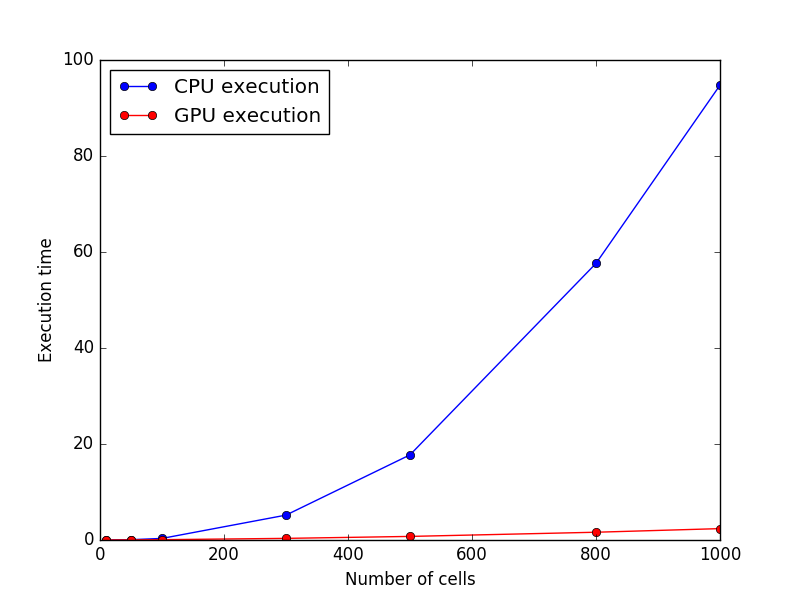
\includegraphics[width=0.8\textwidth]{Images/result_cvg.png}
\caption{A comparison of the computation times of the sequential and parallel execution of the cell merge algorithm.}
\label{res:fig:cvg}
\end{figure}
\begin{figure}[H]
\centering
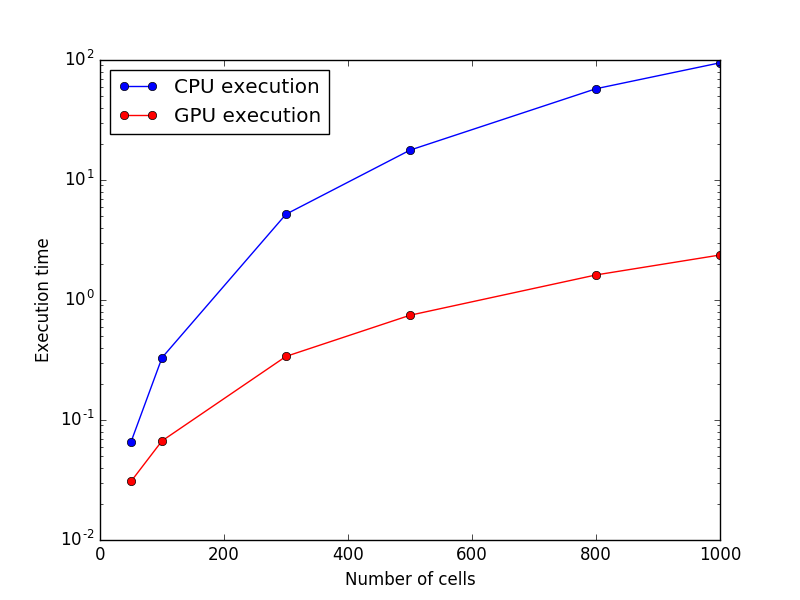
\includegraphics[width=0.8\textwidth]{Images/result_cvg_log.png}
\caption{A logarithmic scale graph of the values depicted in Figure \ref{res:fig:cvg}.}
\label{res:fig:cvg_1og}
\end{figure}
Observing these results it is clear that the GPU outperforms the CPU with its execution time for a higher number of sources. However, for a small number of sources, the overhead costs associated with the set up process before merging can begin on the GPU make it slower than the CPU. Figure \ref{res:fig:speed} shows the speed-up of the parallel merge compared with that of the sequential algorithm. Speed-up is calculated as $speedup = \frac{t_{sequential}}{t_{parallel}}$.
\begin{figure}[H]
\centering
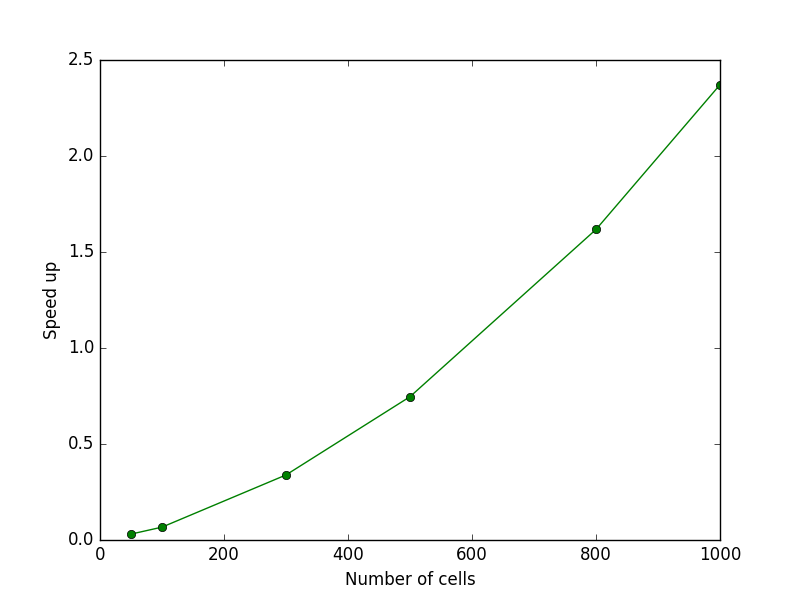
\includegraphics[width=0.8\textwidth]{Images/result_speed.png}
\caption{Speed-up of the parallel process using the execution times illustrated in Figure \ref{res:fig:cvg}.}
\label{res:fig:speed}
\end{figure}
From this, it can be seen that the speed-up increases as the number of sources increases. With 1000 sources, a speed-up of 39.96x is obtained. Given that the average speed-up of a parallel implementation of a process, as stated by \citet{lee2010debunking}, is within an order of magnitude of the sequential process, a speed-up of 39.96x is considered a great improvement in computation time. 
\\
\\
To further analyse the speed-up and provide better insight as to how the parallel implementation operates and what contributes to the speeds obtained, the times for each step of the parallel process was analysed. Figure \ref{res:fig:prof} shows the time taken for each step of the process to execute for a given number of sources.
\begin{figure}[H]
\centering
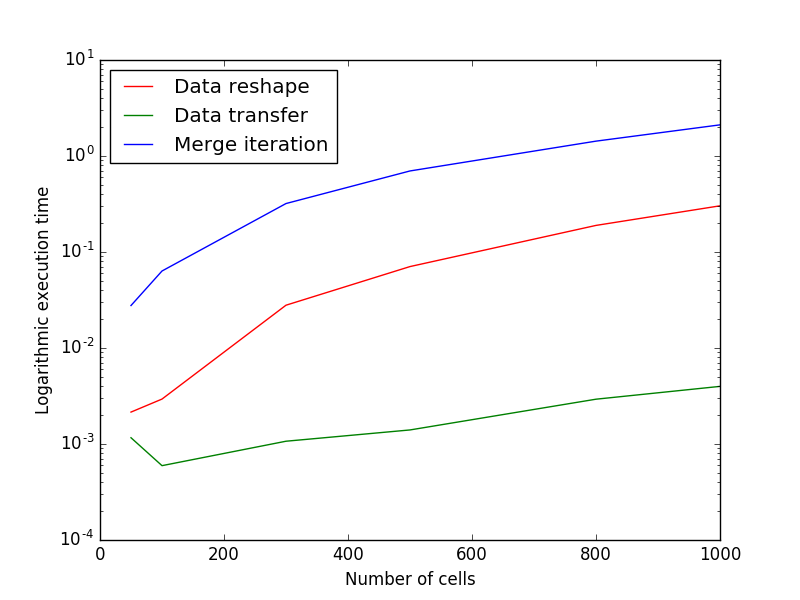
\includegraphics[width=0.8\textwidth]{Images/result_profile.png}
\caption{Breakdown of the time taken for each subprocess in the parallel merge process.}
\label{res:fig:prof}
\end{figure}
Figure \ref{res:fig:prof} shows that, for merges with a smaller number of sources, the transfer time to the GPU is relatively constant, while the merge iteration time and data reshape time scale up appropriately. This constant initial transfer cost is what leads to the sequential process outperforming the parallel for smaller sets of sources. For larger sets of sources, the merge iteration and data reshaping time increases at a much higher rate than that of the data transfer.  This reinforced the parallel implementation as the preferred operation for larger sets of sources.
\\
\\
While the speed-up of the parallel implementation of the cell merge algorithm is noteworthy, it should also be stated that, even with further optimisation, it will only increase to a known theoretical limit. According to \citet{amdahl1967validity}, the maximum speed-up can be calculated as:
\begin{equation}
	speedup = \frac{1}{(1-p)+\frac{p}{s}},
\end{equation}
where $p$ is the percentage of the overall process which can be parallelised and $s$ is the speed-up of the parallelised portion alone. As with all parallel systems, the cell merge is therefore limited to a maximum speed-up.
\\
\\
The leading limitation of the GPU is the availability of memory. Large arrays are created to store the relational data on the GPU. For $n$ sources, the memory requirement to compute the merge is $O(n^2)$ since the \textit{d\_related} and \textit{d\_sources} arrays are $n \times n$ and $n \times n \times 3$, respectively, where each source is initially used as a centre. Therefore, given that the NVIDIA GTX 750 Ti has an internal memory capacity of 2 GB, the maximum number of sources which could be merged on the GPU is restricted to around 7500. This is below the average number of sources for an image generated by a radio telescope which is generally of the order of $\sim$10000 sources. Thus for the parallel algorithm to be of practical use, additional optimisation of the data stored on the GPU will have to be considered.